\section{Network performance experiment design} \label{chap:net_sim}

We now discuss the methodology for the performance portion of the implementation evaluation.
That is, this section focuses on evaluating MQuicTT against the base $rumqtt$ implementation.

The critical consideration for this design is the scenarios in which IoT devices are used.
When evaluating the network performance of the implementations, we considered two options: using real IoT devices or using a network simulation tool.
Due to technical limitations that came with using real devices, such as not being able to access the router of our network, we opted for simulation.
In this section, we will discuss how we used Mininet~\citep{lantz_mininet_2021}, a realistic virtual network, in our evaluation.

Mininet is a tool that network developers and researchers can use to create software-defined networks (SNDs) using the $OpenFlow$ standard.

\begin{figure}[ht]
    \centering
    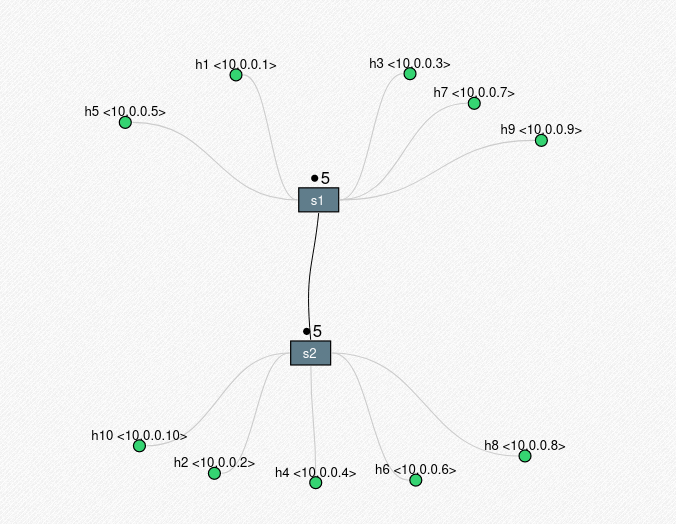
\includegraphics[width=0.9\linewidth]{images/mininet_topo.png}
    \caption{The resulting Dumbbell topology with the broker being h9 - the central node. The link between the central switch and the central host results in a congested network.}
    \label{fig:mininet-topo}
\end{figure}

Using the Python API provided, we created the network topology shown in Figure~\ref{fig:mininet-topo}.
The script takes several parameters to create the following three scenarios:

\begin{itemize}
    \item A synthetic scenario testing the limits of implementations.
    \item A realistic scenario based on a smart-home use-case.
    \item A realistic scenario based on a 3D printer farm.
\end{itemize}

The topology for all three scenarios remains the same - a minimum spanning tree of a typical IoT mesh network.
When designing this topology, we needed it to reflect various realistic IoT scenarios.
We can imagine this as a singular room in a home with all of its smart appliances being a cluster in the smart home or a cluster of 3D printers in a section of a farm in the 3D printer farm.
The critical feature of this topology is that many clusters are connected to a central broker that controls the topology, hence creating a dumbbell structure.
The full definition of this topology can be found in Appendix~\ref{appendix:topo}.
The variables that the script changes between scenarios and simulations are the link's \textit{bandwidth}, \textit{delay} and the rate of \textit{packet loss}.

The bandwidth of a link is the maximum rate of data transfer we can achieve.
In contrast to bandwidth in signal processing, we measure bandwidth in bits per second rather than hertz in computer networking.
The delay of a link specifies the latency of the link.
It is the time that a bit of data takes to travel across a link. 
We measure this in milliseconds.
Link delay corresponds to the geographical distance between the communicating parties; however, in the case of IoT, we can expect devices to be in local proximity.
Lastly, the packet loss rate shows the percentage of corrupted or dropped packets in transit.
Various protocols having to retransmit packets also adds to the delay of data transfer.
Importantly, we have only considered the typical circumstances of packet loss and have not included scenarios such as interference or packet loss attacks.

The bandwidth and delay numbers correspond, as closely as possible, to various link types in a network.
To do so, for the smart-home scenario, we have gathered data from the~\cite{ofcom_uk_2021} report on UK broadband speeds.
There were specific cases in which it was not possible to find this data in the report; hence it was augmented using a similar methodology in work conducted by~\cite{previdi_is-is_2019} and in the case of ZigBee, the work by~\citet{alena_fault_2011}.

\begin{table}[ht]
    \caption{The parameters chosen for each link simulation in Mininet in the smart home scenario. The types of links were chosen as the most commonly occurring ones in IoT use cases.}\label{tab:links:home}
    %\tt 
    \rowcolors{2}{}{gray!3}
    \begin{tabular}{@{}llll@{}}
        \toprule
        \textbf{Simulated Link Type} & \textbf{Link bandwidth (Mb/s)} & \textbf{Link delay (ms)} & \textbf{Packet loss rate (\%)} \\
        Wi-Fi                        & \texttt{30}                    & \texttt{10}              & \texttt{2}                     \\
        ZigBee                       & \texttt{0.25}                  & \texttt{5}               & \texttt{1}                     \\
        4G                           & \texttt{4}                     & \texttt{20}              & \texttt{1.5}                   \\
        3G                           & \texttt{1}                     & \texttt{40}              & \texttt{1.5}                   \\
        100Mb Ethernet               & \texttt{100}                   & \texttt{1}               & \texttt{0.2}                   \\
        \bottomrule
    \end{tabular}
\end{table}

Hence, we expect that the bandwidth and link delay numbers accurately represent a real-world scenario.
However, it was complicated to find exact estimates for packet loss rates, with most sources describing approximations for a stable connection~\citep{sdu_ictp-sdu_2013} and not precise measurements.
Hence, the data are best estimates, cross-validated through the different sources and are not exact values.

In the case of the smart home scenario, as presented in Table~\ref{tab:links:home}, we expect that our packet loss rates are accurate as these, as previously stated, do appear in the home broadband reports and other studies.
In the case of the 3D printer, as presented in Table~\ref{tab:links:3d} farm scenario, due to the number of machines and the interference these cause in a 3D printer farm, we modelled this scenario to have more packet loss.
We specifically chose this scenario to test the benefits that QUIC should receive in an environment with high packet loss.
However, we found it difficult to find exact data on packet loss percentages in smart factories or workshops; hence, we expect a margin of error on some of the values.

In general, we can assume that the packet loss rates will increase by some constant factor across all links.
Hence, we have also created a synthetic scenario with extreme packet loss as presented in Table~\ref{tab:links:synth}.
If the protocol performs well for an extreme scenario, we can expect it to also perform well for packet loss percentages up to that scenario.

\begin{table}[ht]
    \caption{The parameters chosen for each link simulation in Mininet in the 3D printer farm scenario. The data assumes a typical IoT setup where most devices are within local geographical proximity. That is, the devices are communicating with each other within the range of one factory or site, with only the central node communicating with some server.}\label{tab:links:3d}
    %\tt 
    \rowcolors{2}{}{gray!3}
    \begin{tabular}{@{}llll@{}}
        \toprule
        \textbf{Simulated Link Type} & \textbf{Link bandwidth (Mb/s)} & \textbf{Link delay (ms)} & \textbf{Packet loss rate (\%)} \\
        Wi-Fi                        & \texttt{30}                    & \texttt{10}              & \texttt{5}                     \\
        ZigBee                       & \texttt{0.25}                  & \texttt{5}               & \texttt{3}                     \\
        4G                           & \texttt{4}                     & \texttt{20}              & \texttt{2.5}                   \\
        3G                           & \texttt{1}                     & \texttt{40}              & \texttt{2.5}                   \\
        100Mb Ethernet               & \texttt{100}                   & \texttt{1}               & \texttt{0.5}                   \\
        \bottomrule
    \end{tabular}
\end{table}

\begin{table}[ht]
    \caption{The parameters chosen for each link simulation in Mininet in the synthetic scenario. Here we opt for extreme packet loss scenarios to test the boundaries of the protocols. We opted for 20 times the normal packet loss that the link can expect in each case. We have also tested this for higher values however all protocol implementations greatly suffered in performance beyond this.}\label{tab:links:synth}
    %\tt 
    \rowcolors{2}{}{gray!3}
    \begin{tabular}{@{}llll@{}}
        \toprule
        \textbf{Simulated Link Type} & \textbf{Link bandwidth (Mb/s)} & \textbf{Link delay (ms)} & \textbf{Packet loss rate (\%)} \\
        Wi-Fi                        & \texttt{30}                    & \texttt{10}              & \texttt{40}                     \\
        ZigBee                       & \texttt{0.25}                  & \texttt{5}               & \texttt{20}                     \\
        4G                           & \texttt{4}                     & \texttt{20}              & \texttt{30}                   \\
        3G                           & \texttt{1}                     & \texttt{40}              & \texttt{30}                   \\
        100Mb Ethernet               & \texttt{100}                   & \texttt{1}               & \texttt{4}                   \\
        \bottomrule
    \end{tabular}
\end{table}

We evaluate MQuicTT's performance using the presented topologies and respective simulation parameters in the following way.
Each protocol transmits 100 messages from a client to a broker for each data link.

During this, we measure the following:

\begin{itemize}
    \item The time taken for the underlying transport protocol to establish a connection.
    \item The connection time. That is, the time before MQTT can send its first data packet.
    \item The time taken to transmit the message to the broker.
\end{itemize}

This is repeated 10 times, and the average transmission time is taken to ensure accurate results.
This process is repeated for all three testing scenarios.

In general, MQTT allows for messages with a maximum size of approximately 260MB.
However, this is a huge message, and most publicly deployed brokers reject it, so we created a representative message for each use case.
Each topic in MQTT consists of a hierarchy of topic levels separated by a forward slash.
For example, in a smart home scenario, we may have a topic like $home/groundfloor/kitchen/temp$ to control the temperature in the kitchen via a smart thermostat.
A topic may also include a wildcard.
The topic string $home/groundfloor/+/temp$ includes a \textit{single-level} wildcard that will match an arbitrary string.
This would match the topic $home/groundfloor/lounge/temp$, but not match the topic $home/secondfloor/kitchen/temp$.
If a client wishes to subscribe to multiple topics with the same prefix, a \textit{multi-level} wildcard may be used.
For example, the topic $home/secondfloor/kitchen/\#$ can be used to subscribe to all topics with a prefix matching the string before the hash character.
Notably, brokers reserve topics for system messages starting with the \$ character.

The chosen topic and the transmitted message for each scenario can be found in Appendix~\ref{appendix:mqtt_message}.
